\documentclass[a4paper,11pt]{ujreport}

%%【PostScript, JPEG, PNG等の画像の貼り込み】
%% 利用するパッケージを選んでコメントアウトしてください.
\usepackage{graphicx} % for \includegraphics[width=3cm]{sample.eps}
\usepackage{epsfig} % for \psfig{file=sample.eps,width=3cm}
%\usepackage{epsf} % for \epsfile{file=sample.eps,scale=0.6}
%\usepackage{epsbox} % for \epsfile{file=sample.eps,scale=0.6}

\usepackage{times} % use Times Font instead of Computer Modern
% \usepackage{listings} % for soursecode
% \usepackage{plistings} % for soursecode

\setcounter{tocdepth}{3}
\setcounter{page}{-1}

\setlength{\oddsidemargin}{0.1in}
\setlength{\evensidemargin}{0.1in}
\setlength{\topmargin}{0in}
\setlength{\textwidth}{6in}
%\setlength{\textheight}{10.1in}
\setlength{\parskip}{0em}
\setlength{\topsep}{0em}

%\newcommand{\zu}[1]{{\gt \bf 図\ref{#1}}}

%% タイトル生成用パッケージ(重要)
\usepackage{mast-jp-sjis}

%% タイトル
%% 【注意】タイトルの最後に\\ を入れるとエラーになります
\title{NoSQL型データベースシステムでの実体化ビュー選択に関する研究}
%% 著者
\author{髙木 颯汰}
%% 指導教員
\advisor{古瀬 一隆 陳 漢雄}

%% 年月 (提出年月)
%% 年月は必要に応じて書き替えてください.
\majorfield{ } \yearandmonth{2019年 1月}



\begin{document}
\maketitle
\thispagestyle{empty}
\newpage

\thispagestyle{empty}
\vspace*{20pt plus 1fil}
\parindent=1zw
\noindent
%%
%% 論文の概要(Abstract)
%%
\begin{center}
	{\bf 概要}
	\vspace{5mm}
\end{center}
本論文ではNoSQLの一種であるドキュメント指向データベースに実体化ビューを導入する事によって問い合わせ処理を高速化する手法を提案する.ドキュメント指向データベースでは従来のリレーショナルデータベースにあったような参照型のデータ構造に加えて埋込型のデータ構造を選択できる.参照先の内容を埋め込む事によって結合処理をしなくて済むが,ファイルサイズが大きくなる傾向にあり,フラグメンテーションが発生し,逆にパフォーマンスが落ちる可能性がある.そこで本手法ではリレーショナルデータベースで実現されている実体化ビューの概念をNoSQLにも応用する事で,問い合わせ処理を自動的に高速化する.具体的には,頻繁に問い合わせのある結合処理や集計処理を自動的に検知してその部分のみ予め実体化することでデータベースアクセスの高速化を実現している.実体化する箇所の選択を自動化することにより,データベースシステム管理者が行なっていた作業を簡略化し,客観的で正確な実体化ビュー選択が可能となる.

%%%%%
\par
\vspace{0pt plus 1fil}
\newpage

\pagenumbering{roman} % I, II, III, IV
\tableofcontents
\listoffigures
\listoftables

\pagebreak \setcounter{page}{1}
\pagenumbering{arabic} % 1,2,3


\chapter{はじめに}
\label{chap:Introduction}

数年前までは主要なデータストアとして,リレーショナルデータベースがあげられることがほとんどであった.それは多くの開発者がSQLに慣れ親しんでおり,正規化されたデータモデル,トランザクションの必要性,耐久性のあるストレージエンジンが提供する保証を受けられるからである\cite{Sky株式会社201212}.しかし近年高いスケーラビリティや大量なデータ処理が得意であることなどからNoSQLに対する需要が急激に増えている.

例えばNoSQLの一種のドキュメント指向データベースはデータベースの構造を表すスキーマを定義する必要がなく,大量なデータを事前準備なしで格納することができる.従来のリレーショナルデータベースにあったような参照型のデータ構造に加えて埋込型のデータ構造を選択できる.型宣言の必要のないスクリプト言語と相性が良いことなども合間って,プロトタイプを高速に開発することが求められるビジネスの現場で採用されることが増えている\cite{渡部201602}.

一方でドキュメント指向データベースの特徴とも言える階層的なデータモデルが更新処理速度の低下やデータ参照の柔軟性を低下を招くことがある.これを防ぐためにはドキュメントに階層的に埋め込むフィールドを適切に選択する必要がある.本論文ではこの選択の自動化し,ドキュメント指向データベースのデータモデルのチューニングを行い,データアクセスを高速化する.

本論文の構成は以下の通りである.まず,第\ref{chap:LiteratureReview}章において関連研究について紹介する.次に,第\ref{chap:ProposedAlgorithm}章において本研究の提案手法について説明をし,第\ref{chap:Experiment}章にて提案手法に関する実験を行い,提案手法の有効性を確める.第\ref{chap:Result}章において実験の結果と考察を述べ,最後に第\ref{chap:Conclusion}章において本論文のまとめと今後の課題を示す.

\chapter{関連技術}
\label{chap:LiteratureReview}
\section{Materialized View}
リレーショナルデータベースにおけるビュー (view) はリレーショナルデータモデルの発案者であるコッドにより導入された概念であり\cite{Codd1974RecentII},1つ以上の表(または他のビュー)から任意のデータを選択し,それらを表したものである.ビューの実体はデータを持たないSQL文であり,実行された際にはバックグラウンドでSELECT処理が毎回実行される.それに対して実体化ビュー(Materialized View)はビューと同じく複数の表の結合処理や集計処理を行うが,その結果を実際のテーブルに保持する.保持された実体化ビューは元のテーブルが更新されるたびに更新される.そのため,最新でない状態を取得する可能性はあるが,結合処理が必要ないため効率的なアクセスが可能になる.その一方,更新処理が増加するので実体化ビュー化する部分の選択は慎重に行う必要があり,この作業を自動化する研究が行われている\cite{mistry2001materialized}.図\ref{figure:MvDescription}は1対1のデータモデルの実体化ビューを図示したものである.
\begin{figure}[htbp]
	\begin{center}
		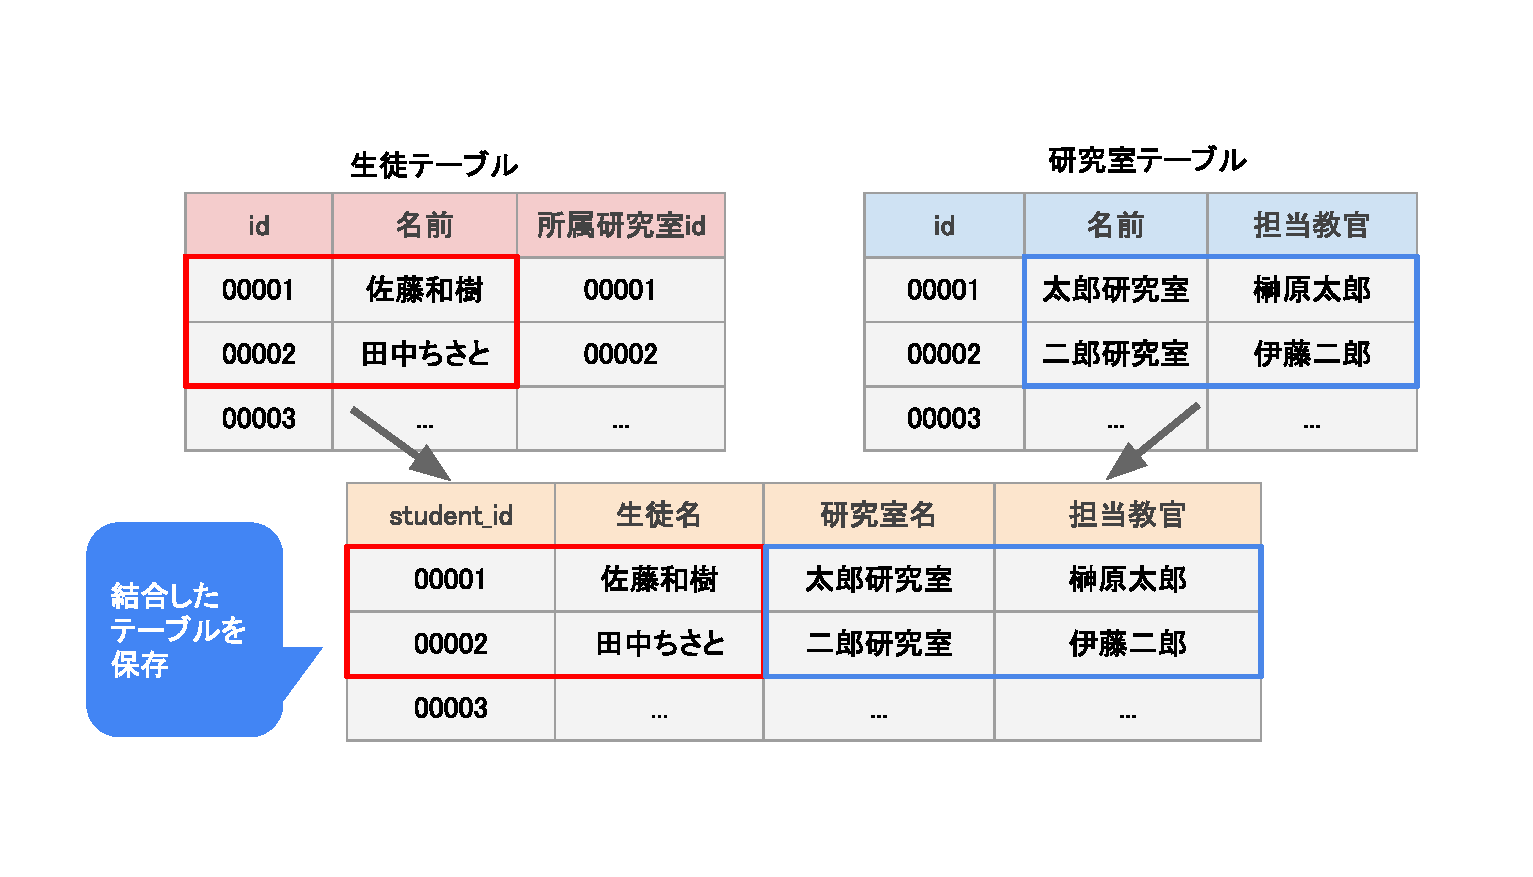
\includegraphics[width=32em, trim=0 5em 0 0]{src/MvDescription.eps} %[trim=left bottom right top]
	\end{center}
	\caption{実体化ビュー}
	\label{figure:MvDescription}
\end{figure}


多対多の結合を表す際には中間テーブルを用意してそれぞれのテーブルからレコードを結合する.その際の流れを図\ref{figure:MvDescription2}に示す.履修中間テーブルに生徒idと授業idを格納している.idが00001の生徒が履修している授業を取得する際には履修中間テーブルのstudent\_idが00001のレコードを取得し,付随するclass\_idを用いて授業の情報を取得する.結合元のテーブルのレコード数が無数にある場合には結合元テーブルでの検索時間が増加し,結合元のテーブルのレコード数の増加と共に中間テーブルのレコード数も増える傾向にあるので,中間テーブルでの検索時間も増加する.
\begin{figure}[htbp]
	\begin{center}
		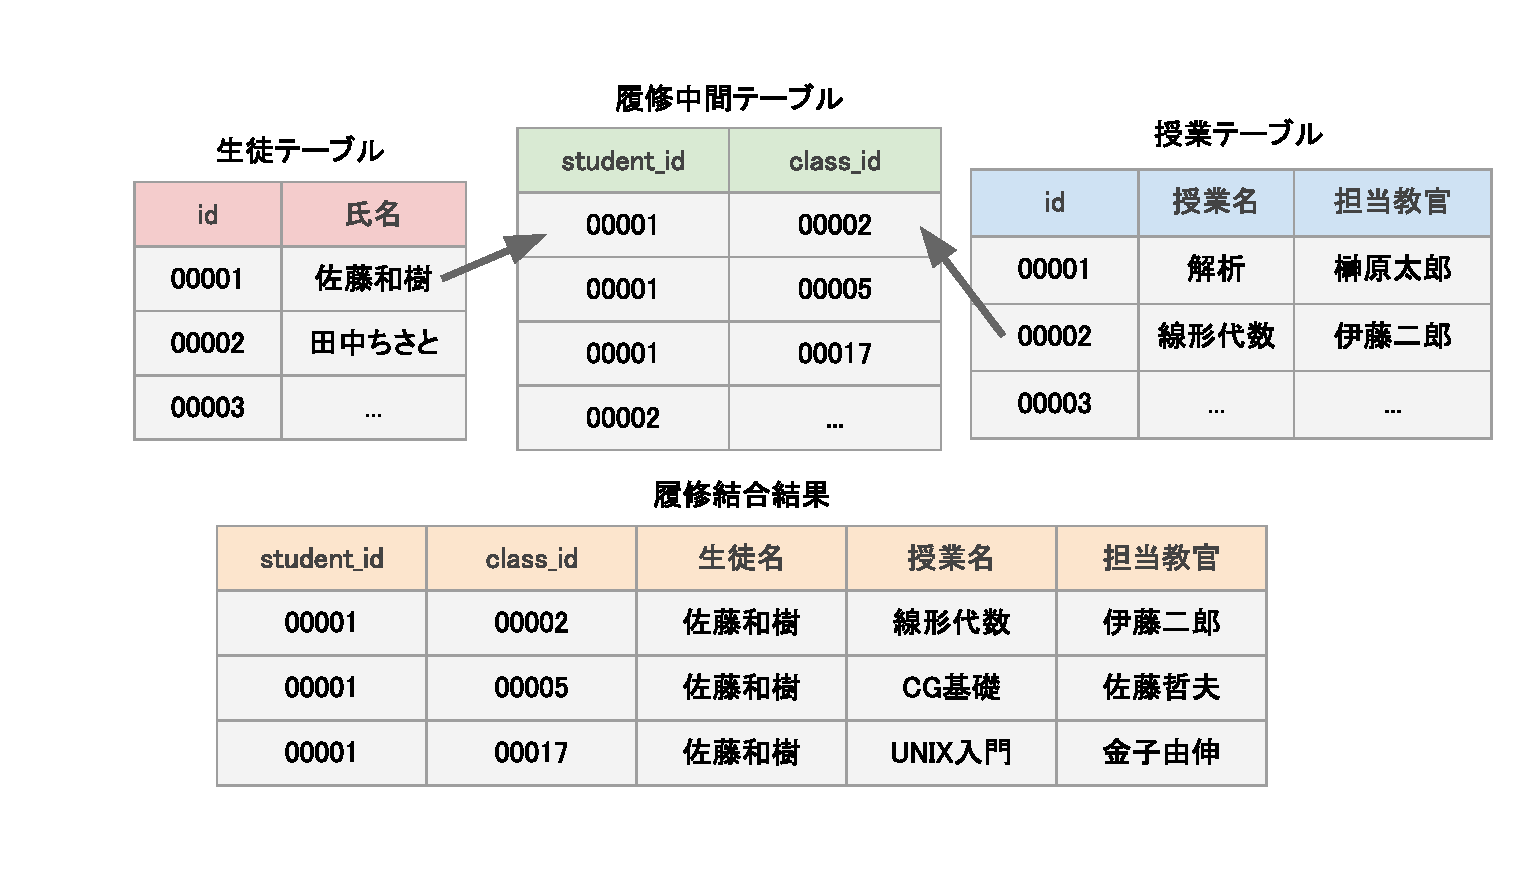
\includegraphics[width=32em, trim=0 5em 0 0]{src/MvDescription2.eps} %[trim=left bottom right top]
	\end{center}
	\caption{多対多の結合}
	\label{figure:MvDescription2}
\end{figure}
Materialized Viewを用いた際のメリットとして,結合処理や集計処理が不要になり高速化することに加え,問い合わせに用いるSQL文が簡素化することが挙げられる.表\ref{table:mv_sql}は図\ref{figure:MvDescription2}の生徒テーブルをstudent,授業テーブルをclass,履修中間テーブルをcourse\_selection,生徒の履修結合結果を得るために作成したMaterialized Viewをmv\_course\_selectionとした際に,idが00001の生徒が履修している授業を取得するSQL文をMaterialized Viewを使用する場合としない場合を比較したものである.
\begin{table}[htb]
  \begin{center}
    \caption{生徒テーブルと授業テーブルを結合するSQL}
		\label{table:mv_sql}
    \begin{tabular}{|l|l|} \hline
			\begin{tabular}{l}
				Materialized Viewを\\使用しない
			\end{tabular} &
			\begin{tabular}{l}
				SELECT student.id AS student\_id,
				class.id AS class\_id,\\
				student.name AS student\_name,
				class.name AS class\_name,\\
				class.teacher AS teacher\\
				FROM student, class, course\_selection \\
				WHERE course\_selection.student\_id = 00001 AND\\ course\_selection.student\_id = student.id AND\\ course\_selection.class\_id = class.id;\\
			\end{tabular}\\
			 \hline
			 \begin{tabular}{l}
 				Materialized Viewを\\使用する
 			\end{tabular} &
			\begin{tabular}{l}
				SELECT student\_id, class\_id, student\_name, class\_name, teacher\\
				FROM mv\_course\_selection\\
				WHERE student\_id = 00001;
			\end{tabular}
			\\ \hline
    \end{tabular}
  \end{center}
\end{table}

\section{NoSQL}
NoSQLとは,“Not only SQL”の略称であり,SQLを用いないデータベースの総称を表す \cite{太田201204}.情報の大規模化が進み,ビッグデータと呼ばれる概念が登場すると共に,構造が複雑な様々なデータが登場するようになった.NoSQLは,そのような複雑な構造のデータに柔軟に対応し処理を行うことができる.GoogleやAmazon,Twitterなど,世界的規模を誇る企業がNoSQLデータベースを利用しており,今後ますますデータの大規模化が進む現代社会において,重要な役割を果たすデータベースである\cite{太田201204}.
NoSQLデータベースはキー・バリュー型,カラム指向型,ドキュメント指向型,グラフ型の4種類の型に大別することができる.キー・バリュー型は,インデックスであるキーと値であるバリューのペアでデータが構成され,キーを指定することでデータを呼び出すことができる.カラム指向型は行に対してキーが付され,それが複数の列(カラム)に対応する形のデータモデルである.ドキュメント指向型は,JSONやXMLなどの形式で記述されたドキュメントの形でデータを扱うデータモデルである.グラフ型は,データ間の関係性をグラフの構造で表すデータモデルである\cite{太田201204}.

\section{MongoDB}
MongoDBとは,JSONやXMLなどの形式で記述されたドキュメント指向型のデータを扱うNoSQLデータベースの代表的なものの一つである.RDBとは違い,スキーマの定義を必要としない\cite{太田201204}\cite{mongodb}.また,JSON形式のデータを扱うため,Webシステムなどに利用しやすい.
MongoDBにおいては,RDBのテーブルにあたるものとしてコレクション,RDBの行にあたるものとしてドキュメント,RDBの列にあたるものとしてフィールドというデータ構想が使われる.

MongoDBではデータの格納にJSONをバイナリエンコーディングしたBSON形式を用いる\cite{Harrison201512}.RDBMSとMongoDBにおける一般的な検索のクエリを表\ref{table:RDB_Mongo_Find}に,更新のクエリを表\ref{table:RDB_Mongo_Update}に示す.
また,MongoDBはクエリの結果をJSON形式で返す.返却されるクエリセットの例を図\ref{MongoJson}に示す.
\begin{table}[htb]
  \begin{center}
    \caption{RDBMSとMongoDBにおける検索クエリ}
		\label{table:RDB_Mongo_Find}
    \begin{tabular}{|c|l|} \hline
			RDBMS & SELECT * FROM comments WHERE story = "Next Generations";\\ \hline
			MongoDB & db.comments.find(\{story: "Next Generations"\});\\ \hline
    \end{tabular}
  \end{center}
\end{table}
\begin{table}[htb]
  \begin{center}
    \caption{RDBMSとMongoDBにおける更新クエリ}
		\label{table:RDB_Mongo_Update}
    \begin{tabular}{|c|l|} \hline
			RDBMS & UPDATE comments SET story = "Next Generations 2" WHERE story = "Next Generations";\\ \hline
			MongoDB & db.comments.update(\{story: "Next Generations"\}, \{\$set: \{story: "Next Generations 2"\}\});\\ \hline
    \end{tabular}
  \end{center}
\end{table}

\begin{figure}[htbp]
	\begin{center}
		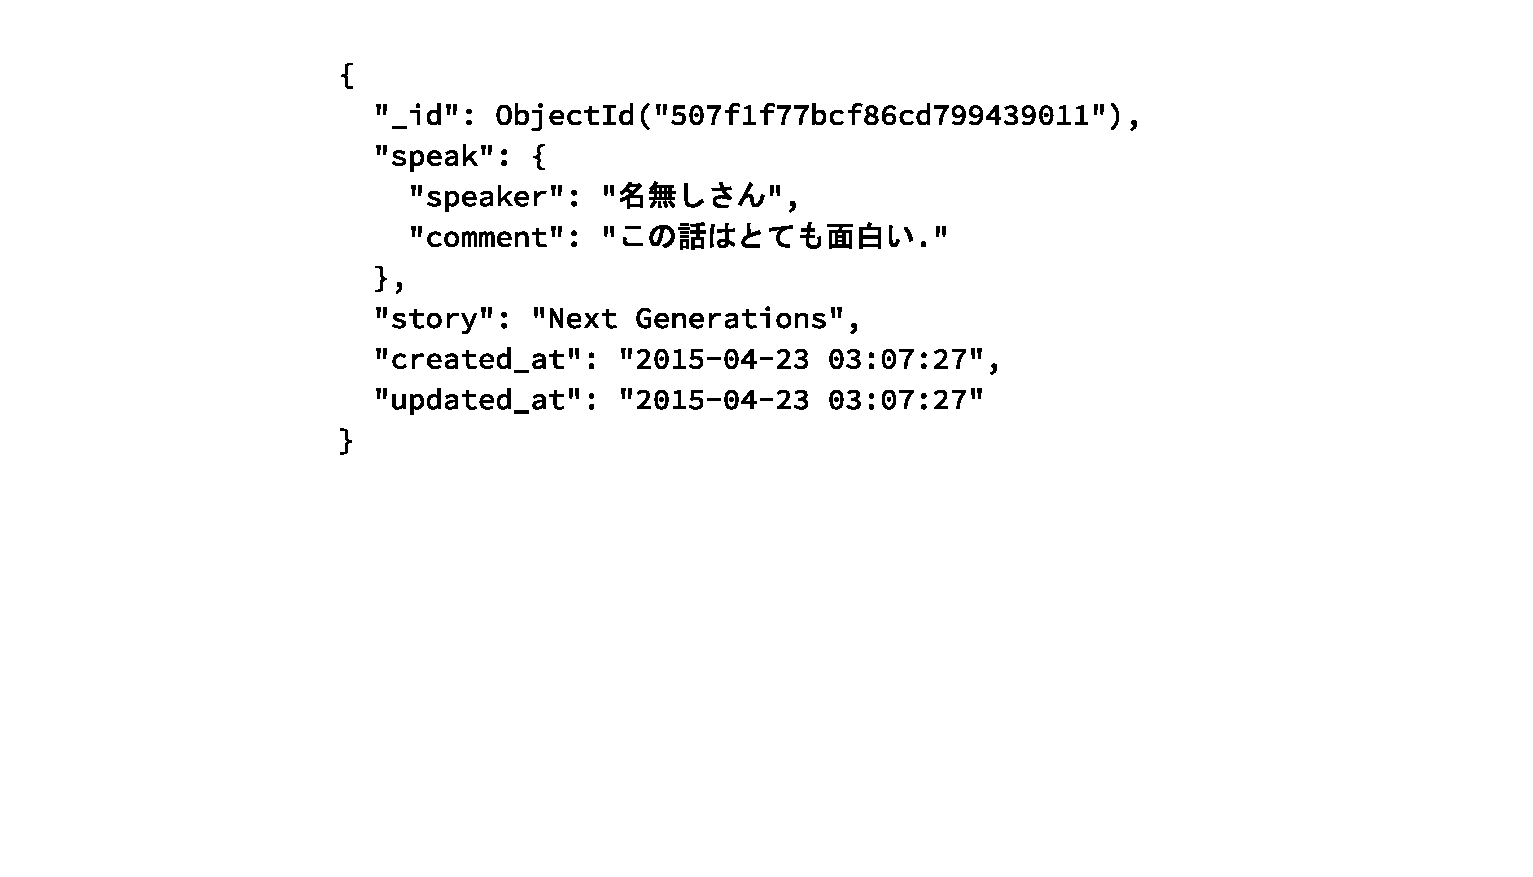
\includegraphics[width=30em, trim=10em 18em 10em 0em]{src/MongoJson.eps} %[trim=left bottom right top]
	\end{center}
	\caption{MongoDBから返されるクエリセットの例}
	\label{MongoJson}
\end{figure}



\section{Restful API}
RESTとはRoy Fieldingが提唱した概念であり\cite{fielding2000architectural},“REpresentational State Transfer”の略である.分散システムにおける複数のソフトウェアを連携させるのに適した考え方であり,やりとりされる情報はそれ自体で完結して解釈できるステートレス性,全てのリソースが一意的なアドレスを持つアドレス可能性,他の基盤的な機能を用いずに別の情報や状態を含むことで他のリソースを参照できる持続性,HTTPメソッド(“GET”や“POST”など)の統一インターフェースを提供していることなどの原則から成る.RESTの原則に則り構築されたHTTPの呼び出しインターフェースをRESTful APIと呼ぶ.本論文ではRESTful APIをミドルウェアに実装し実験を行う.

\chapter{提案手法}
\label{chap:ProposedAlgorithm}
\section{ドキュメント指向型データベースにおける実体化について}
ドキュメント指向型データベースの特徴として埋め込み(embed)がある.従来のRDBでは複数の表による1対多や多対多の関係を表す際に,参照先のプライマリーキーのみを保存してSELECTされる際に結合処理を行う.それに対してドキュメント指向型データベースでは参照先の実データを参照元に埋め込むことができ,これによって結合処理を省くことができる.埋め込み先が複数の場合には更新処理が増加し,従来の参照型に比べてデータアクセスの柔軟性が損なわれるというデメリットがある\cite{Sky株式会社201212}.図\ref{figure:Reference}はドキュメント指向型データベースの参照型を,図\ref{figure:Embed}は図\ref{figure:Reference}のデータを埋込型で表した図である.
また.図\ref{figure:Embed}と図\ref{figure:Reference}のドキュメントを得るためのクエリを表\ref{table:MongoReferenceEmbedFind}に示す.idが123456のドキュメントを更新するクエリを表\ref{table:MongoReferenceEmbedUpdate}に示す.なお,表\ref{table:MongoReferenceEmbedUpdate}の埋込型に関しては,埋め込まれているコレクション全てに対してクエリを実行する必要がある.
\begin{figure}[htbp]
	\begin{center}
		\includegraphics[width=30em, trim=0 5em 0 2em]{src/Reference.eps} %[trim=left bottom right top]
	\end{center}
	\caption{参照型}
	\label{figure:Reference}
\end{figure}
\begin{figure}[htbp]
	\begin{center}
		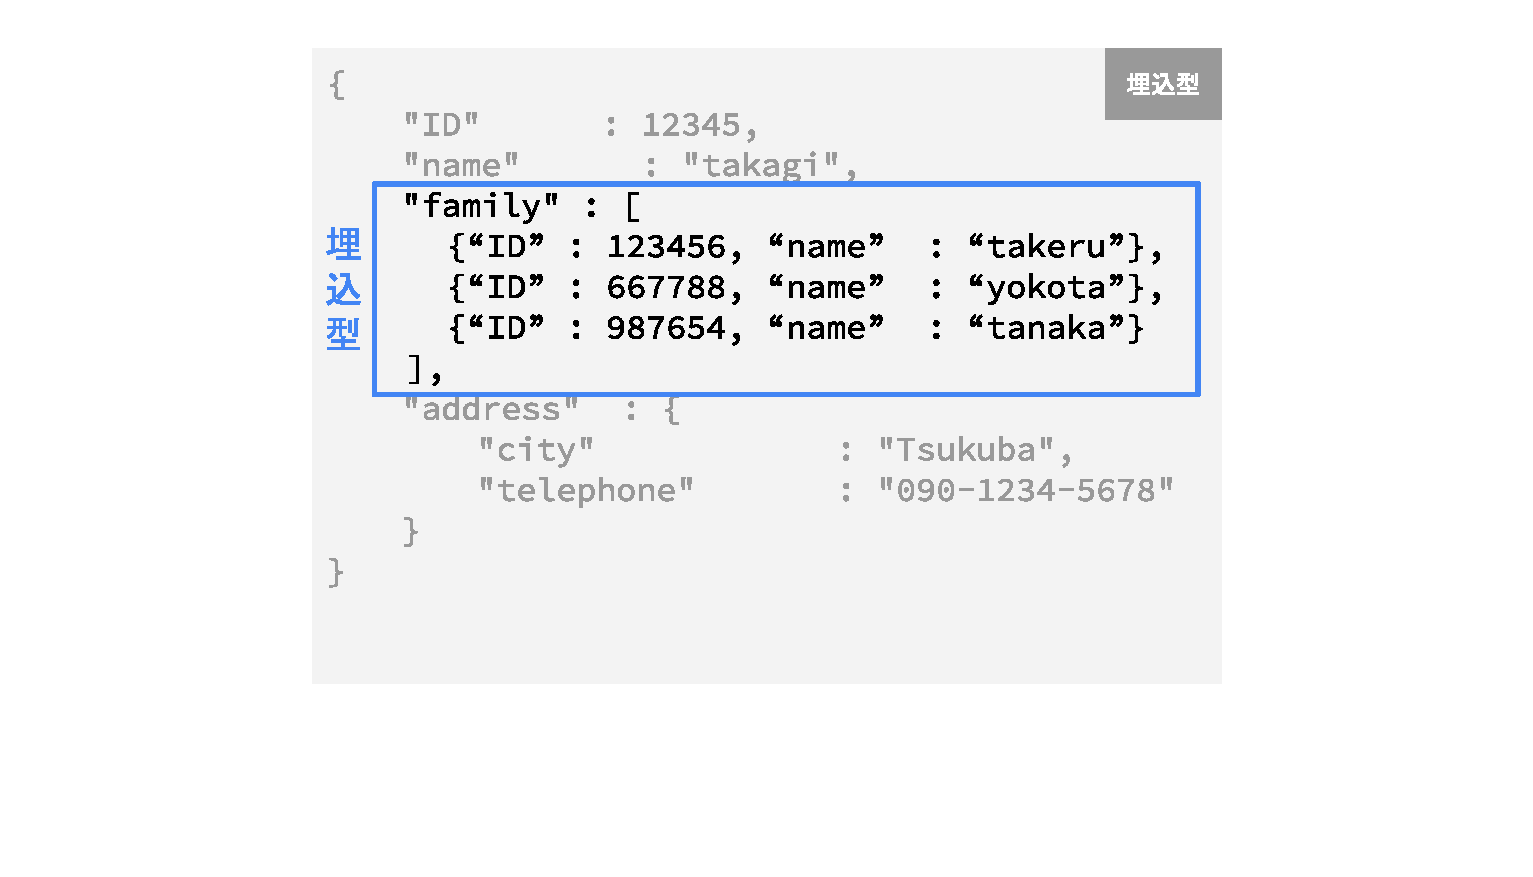
\includegraphics[width=30em, trim=0 7em 0 0em]{src/Embed.eps} %[trim=left bottom right top]
	\end{center}
	\caption{埋込型}
	\label{figure:Embed}
\end{figure}

\begin{table}[htb]
  \begin{center}
    \caption{MongoDBにおける参照型データモデルと埋込型データモデルでの検索クエリ}
		\label{table:MongoReferenceEmbedFind}
    \begin{tabular}{|c|l|} \hline
			参照型 &
			\begin{tabular}{l}
				db.people.aggregate([\{ \$match: \{ID: 12345\}\},\\ \{ \$lookup: \{ from: "families", localField: "familyID", foreignField: "ID"\}\}]);
			\end{tabular}\\ \hline
			埋込型 & db.people.find(\{ID: 12345\});\\ \hline
    \end{tabular}
  \end{center}
\end{table}
\begin{table}[htb]
  \begin{center}
    \caption{MongoDBにおける参照型データモデルと埋込型データモデルでの更新クエリ}
		\label{table:MongoReferenceEmbedUpdate}
    \begin{tabular}{|c|l|} \hline
			参照型 &
			\begin{tabular}{l}
				db.family.update(\{ ID: 123456\},\{ \$set: \{ name: "takebayashi"\}\});
			\end{tabular}\\ \hline
			埋込型 & db.people.update(\{"family.ID": 12345\}, \{ \$set: \{family.\$.name: "takebayashi"\}\});\\ \hline
    \end{tabular}
  \end{center}
\end{table}

全てのドキュメントを埋め込み型として保存すると埋め込み先のドキュメントの更新処理が増え,著しく更新時間が増加する為,データモデルとして最適とは言えない.埋め込み型のデータモデルとして保存するコレクションを最適に選択し,データモデルを最適化することがドキュメント指向型データベースを高速に使用することに繋がる.本論文ではこのコレクションの選択を自動化する.

\section{提案手法の構成}
本論文ではドキュメント指向型データベースの埋込型データモデルをリレーショナルデータベースの実体化ビューと置き換えて考える.ドキュメント指向型データベースのよくアクセスされる部分や処理速度がネックとなっている部分を埋込型として別コレクションに保持することで“実体化ビュー作成”,どの部分を埋込型にするかの判断を“実体化ビュー選択”とする.図\ref{figure:ReferenceToEmbed}は本論文での“実体化ビュー作成”を示したものである.
\begin{figure}[htbp]
	\begin{center}
		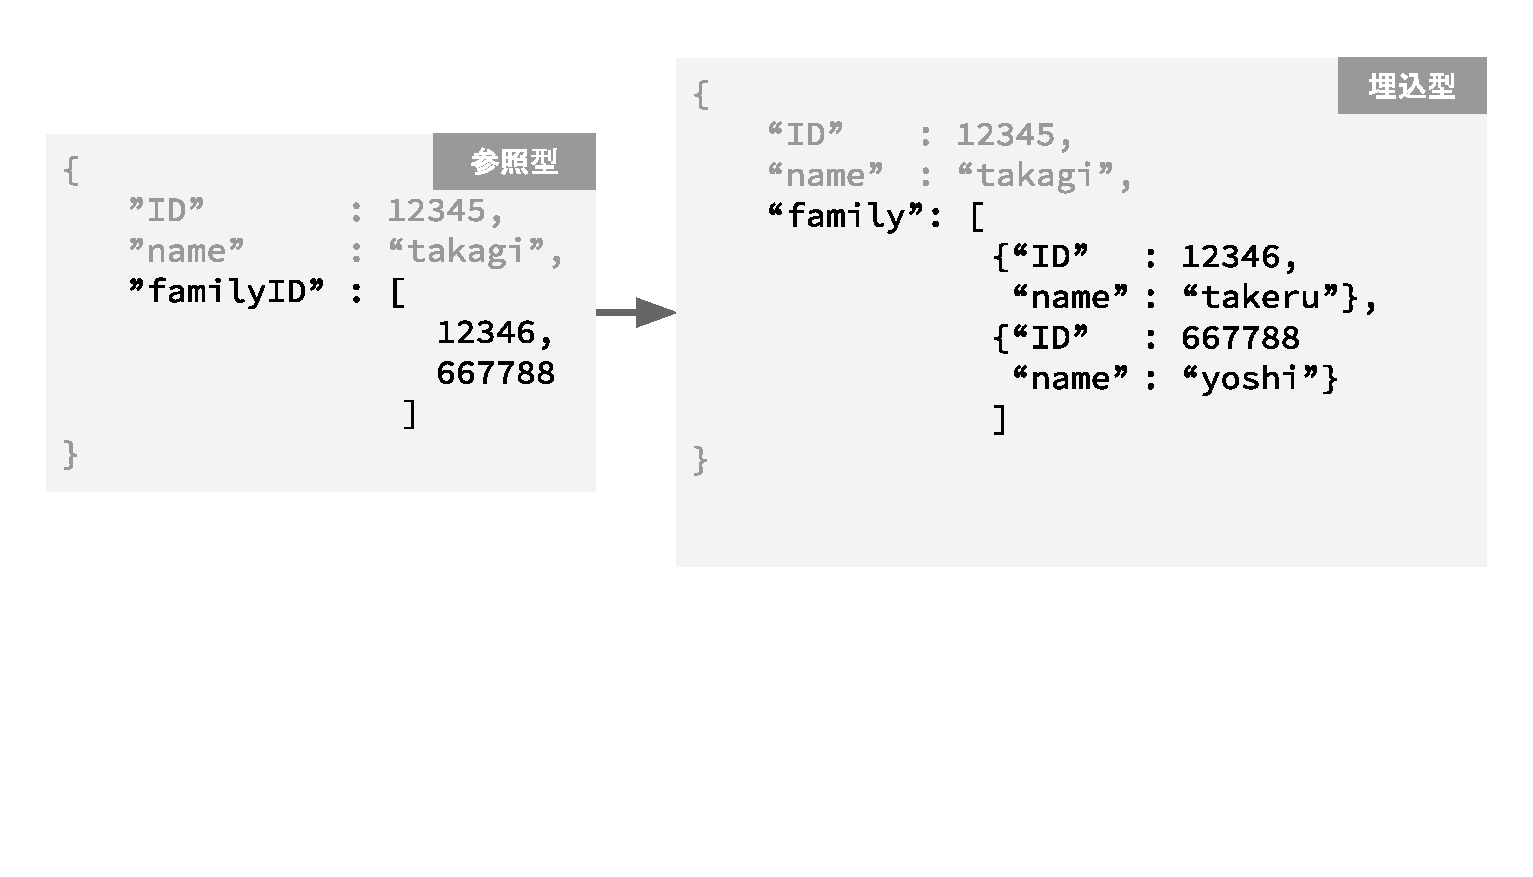
\includegraphics[width=30em, trim=0 13em 0 0]{src/ReferenceToEmbed.eps} %[trim=left bottom right top]
	\end{center}
	\caption{参照型から埋込型への書き換え}
	\label{figure:ReferenceToEmbed}
\end{figure}

実装システムについて図\ref{figure:Midleware}に示す.ユーザーからのデータアクセスから実体化ビュー作成までの流れを図\ref{figure:Midleware}を用いて説明する.
\begin{figure}[h]
	\begin{center}
		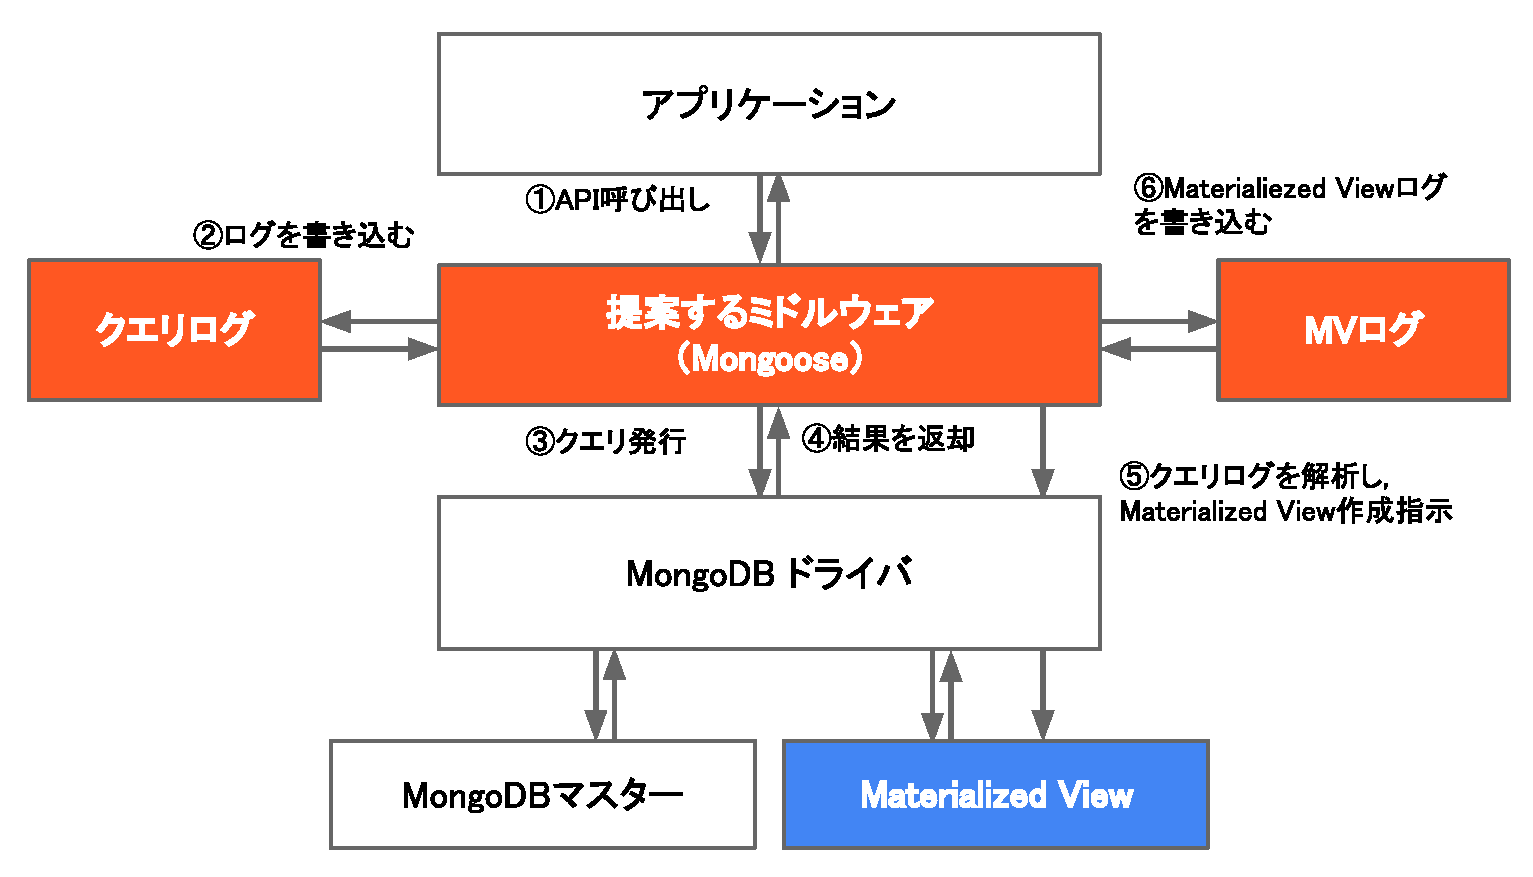
\includegraphics[width=30em]{src/Midleware.eps}
	\end{center}
	\caption{提案ミドルウェア(実体化前)}
	\label{figure:Midleware}
\end{figure}
図\ref{figure:Midleware}-①まずユーザーがアプリケーションからミドルウェアに対してデータアクセスの要求する.図\ref{figure:Midleware}-②ミドルウェアでは,頻繁にアクセスされるドキュメントを分析するために,クエリに関するログを残す.図\ref{figure:Midleware}-③次にMongoDBに対してクエリを発行する.図\ref{figure:Midleware}-④MongoDBから返ってきたクエリセットをアプリケーションに返却する.図\ref{figure:Midleware}-⑤クエリログを解析し,ボトルネックとなっているところや呼び出し回数の多い条件の実体化ビューを作成する.図\ref{figure:Midleware}-⑥実体化したドキュメントに関してログに記録する.

実体化した後のデータアクセスの流れを図\ref{figure:MidlewareMv}に示す.図\ref{figure:MidlewareMv}-①’アプリケーションからデータベースにアクセスがあった場合,まずログからアクセスされたデータが実体化されているか判定する.図\ref{figure:MidlewareMv}-②’実体化されている場合はクエリを書き換えて実体化ビューから結果を取得する.図\ref{figure:MidlewareMv}-③’アプリケーションに結果を返す際には元のクエリに合うように適宜変換する.
\begin{figure}[htbp]
	\begin{center}
		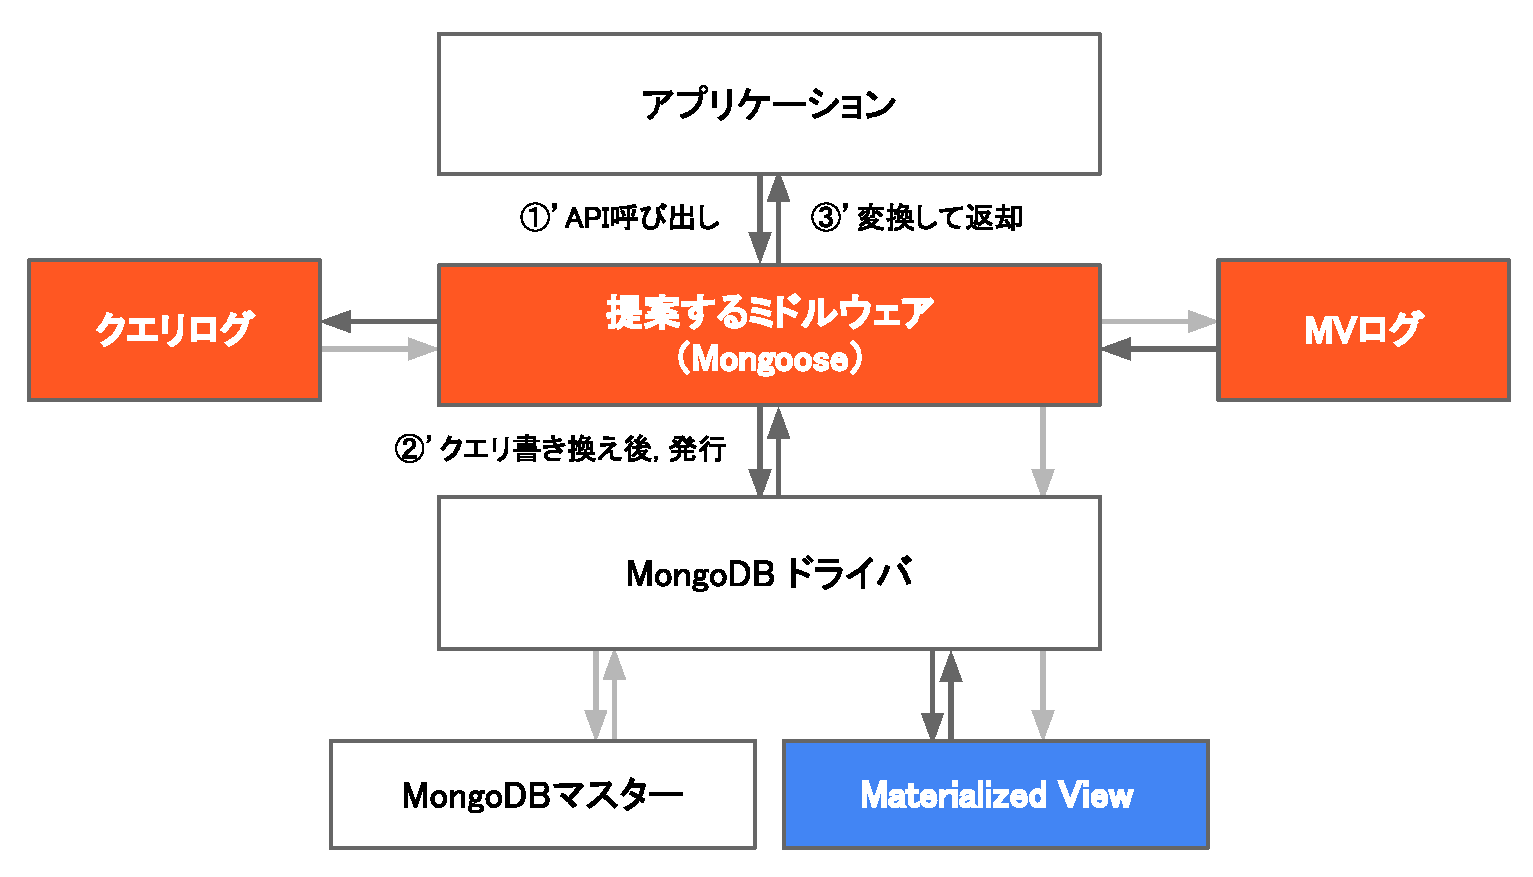
\includegraphics[width=30em]{src/MidlewareMv.eps} %[trim=left bottom right top]
	\end{center}
	\caption{提案ミドルウェア(実体化後)}
	\label{figure:MidlewareMv}
\end{figure}

\section{実体化アルゴリズムについて}
クエリログから実体化するコレクションを決定する条件を適切に設定することで,実体化ビュー選択を自動化することができる.この実体化条件については以下の条件が考えられる.
\begin{enumerate}
  \item クエリログの統計
  \item ドキュメント内の参照数
\end{enumerate}
1の条件は実際のクエリの検索回数・更新回数やその処理時間を元に実体化するコレクションを選定する.2の条件ではドキュメント内の他コレクションへの参照数を元に実体化後の更新処理の増加を予想し,実体化するコレクションを選定する.本論文では更新処理が用意であり,クエリに柔軟に対応できるクエリログの統計を元に実体化する条件を作成する.

\section{逆実体化アルゴリズムについて}
クエリのログを元に実体化した場合,クエリの傾向が変わることで実体化していない状態の方が望ましくなる可能性や,コレクションの特性によっては実体化によるメリットがデメリットより少ない可能性がある.そのような事を防ぐために,定期的に実体化したコレクションに対してもメンテナンスを行い,場合によっては実体化したコレクションをオリジナルのデータモデルに戻すことが必要である.本論文では実体化したコレクションのデータモデルを元に戻す事を逆実体化と定義する.この逆実体化に対しても実体化同様,適切な逆実体化条件を設定する必要がある.

本論文ではクエリのログの統計から実体化後の検索処理時間と更新処理時間を比較し,各コレクションに対して逆実体化の必要性を確認する.

\chapter{実験}
\label{chap:Experiment}
\section{Mongooseについて}
MongooseとはMongoDB用モデリングツールで,Node.jsの非同期環境でうまく動作することを目的として設計されている.Mongooseを使用すれば,モデルを定義して操作することで,MongoDBのコレクション/ドキュメントを操作できる\cite{mongoose}.本論文ではMongooseを用いてMongoDBを操作するミドルウェアを実装する.

\section{実験環境}
実験環境に関する情報を表\ref{table:experiment_env}に示す.
\begin{table}[htb]
  \begin{center}
    \caption{実験環境}
		\label{table:experiment_env}
    \begin{tabular}{|c|c|} \hline
      マシン & MacBook (Retina, 12-inch, 2017) \\ \hline
      プロセッサ & 1.2 GHz Intel Core m3\\ \hline
      メモリ & 8 GB 1867 MHz LPDDR3\\ \hline
      データベースシステム & Mongodb version 3.1.10\\ \hline
    \end{tabular}
  \end{center}
\end{table}

\section{実験方法}
本論文の実験で用いたコレクションはpersonコレクション,storyコレクション,commentコレクション,publisherコレクションである.コレクションの構造,コレクション同士の参照に関しては図\ref{ExperimentCollection},図\ref{ExperimentCollection2}に示す.storyコレクションには筆者として1つのpersonドキュメントのidを格納する.このstoryドキュメントが検索された際には筆者のidをperosnコレクションから検索し,結合して結果を返す.同じようにファンとしてpersonドキュメントのidを配列で格納することで複数のpersonドキュメントをstoryドキュメントに埋め込む.実際の実験データではファンとして100のpersonドキュメントのidを埋め込む.その際,100回結合処理を実行することになる.出版社としてpublisherドキュメントのidも格納する.
\begin{figure}[htbp]
	\begin{center}
		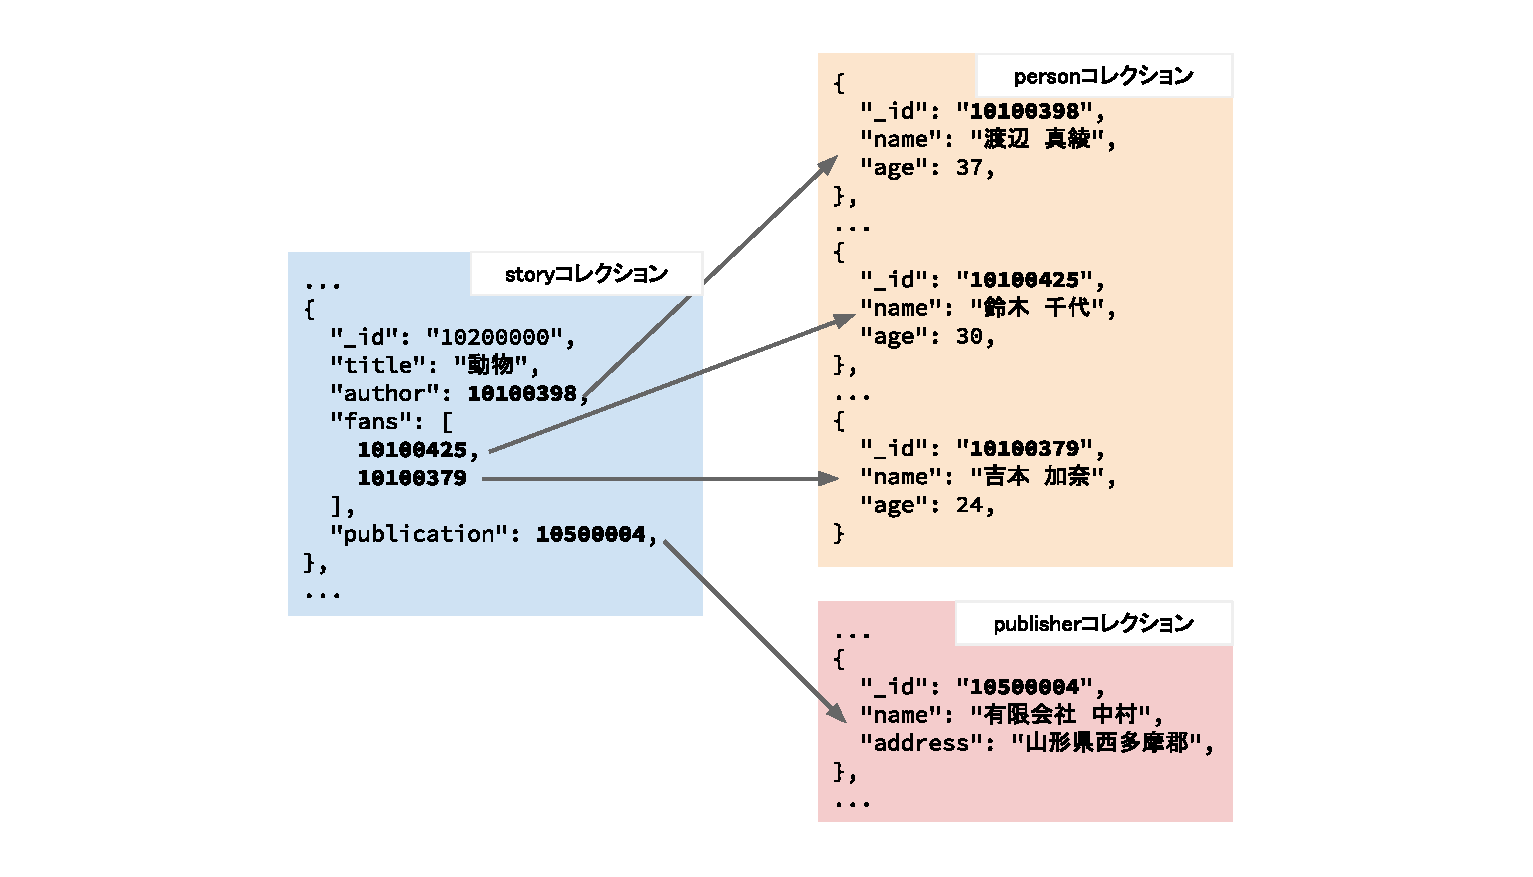
\includegraphics[width=30em, trim=10em 2em 10em 2em]{src/ExperimentCollection.eps} %[trim=left bottom right top]
	\end{center}
	\caption{storyコレクションから各コレクションへの参照}
	\label{ExperimentCollection}
\end{figure}
\begin{figure}[htbp]
	\begin{center}
		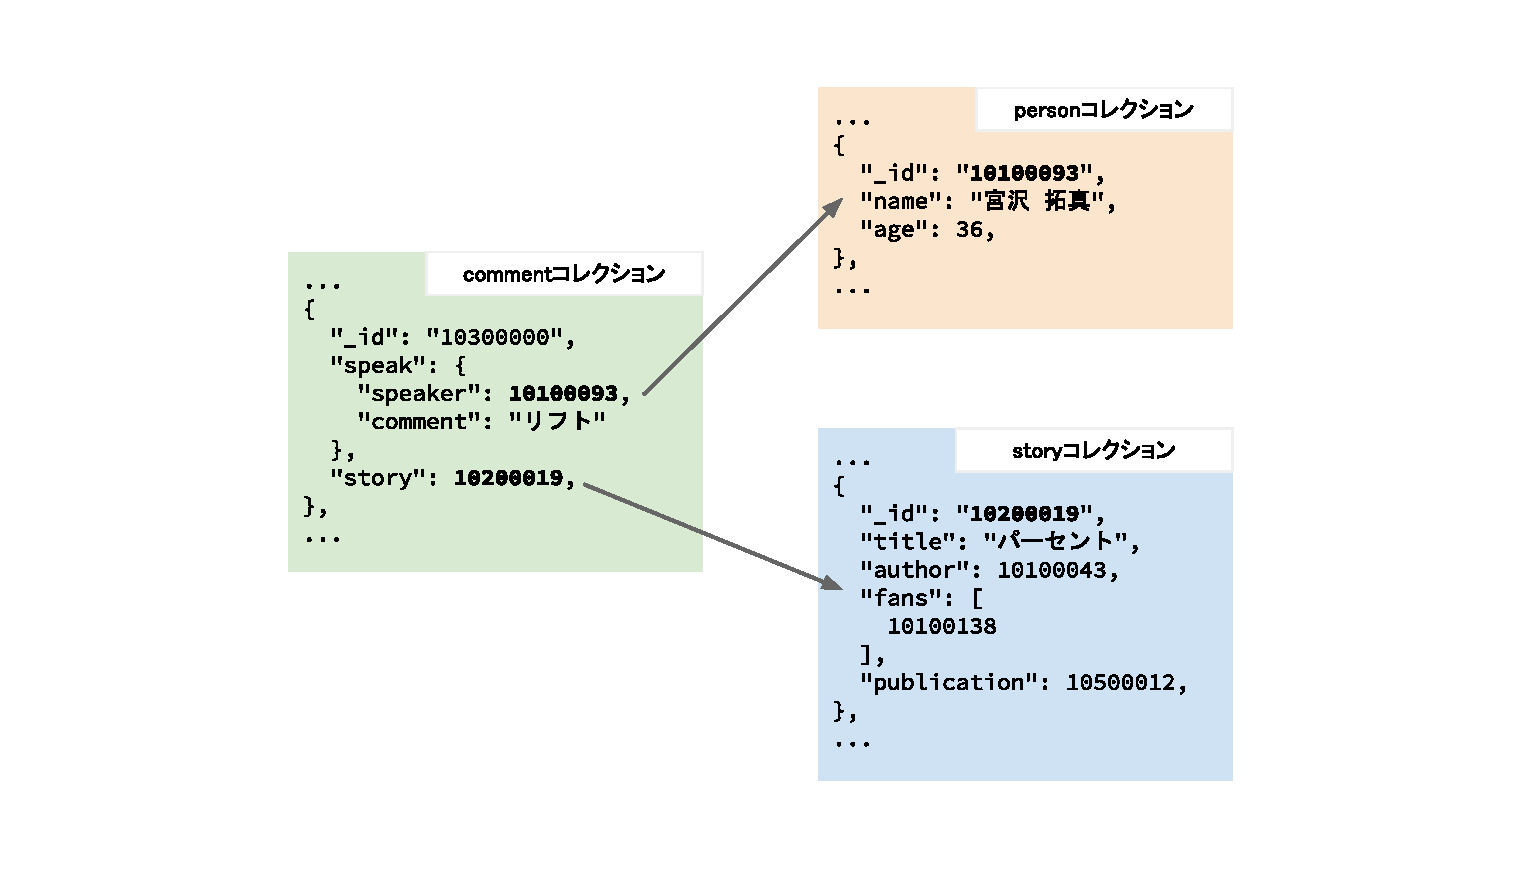
\includegraphics[width=30em, trim=10em 2em 10em 2em]{src/ExperimentCollection2.eps} %[trim=left bottom right top]
	\end{center}
	\caption{commentコレクションから各コレクションへの参照}
	\label{ExperimentCollection2}
\end{figure}
実験において使用するデータは全て参照型のデータモデルで挿入する.実体化していない状態で検索された場合には結合処理を行い結果を返す.実験に用いるドキュメントはPythonのライブラリであるfaker\cite{faker}を用いて作成した.各コレクションに対して1000ドキュメントを作成した.


実験では全てのコレクションが従来の参照型のデータモデルを用いたシステムと実体化条件を用いずに全てのコレクションを実体化したシステム,実体化条件を用いて適宜コレクションを実体化するシステムの3つのデータベースシステムを比較する.その際,実体化を用いたシステムでは検索や更新を提案ミドルウェアを用いて処理する.

この3つのシステムを比較する際,検索と更新の比率を変えた4つのクエリパターンを用いて行う.このクエリパターンを表に示す.このパターンを用いて実験A~Dを行う.
\begin{table}[htb]
  \begin{center}
    \caption{クエリパターン}
		\label{table:experiment_query_pattern}
    \begin{tabular}{|c|c|c|} \hline
        & 検索回数 & 更新回数 \\ \hline
      パターンA & 99 & 1\\ \hline
      パターンB & 97 & 3\\ \hline
			パターンC & 95 & 5\\ \hline
      パターンD & 90 & 10\\ \hline
    \end{tabular}
  \end{center}
\end{table}
それぞれのパターンに対して,使用したクエリを表で示す.ここではMongooseのpopulateを用いて結合処理をおこなっている.また,提案手法を用いる場合には検索・更新に関わらずクエリが5回処理された際に実体化条件を検討し,適宜実体化ビューを作成,破棄を行う.
\begin{table}[htb]
  \begin{center}
    \caption{実験で使用した検索クエリ}
		\label{table:ExperimentFindQuery}
    \begin{tabular}{|c|c|} \hline
      コレクション & クエリ\\ \hline
      person & db.person.find(\{\_id: testID\})populate([]);\\ \hline
			story & db.story.find(\{\_id: testID\}).populate(["author", "fans", "publication", "comments"]);\\ \hline
      comment & db.comment.find(\{\_id: testID\}).populate(["speak.speaker", "story"]);\\ \hline
      publisher & db.publisher.find(\{\_id: testID\}).populate([]);\\ \hline
    \end{tabular}
  \end{center}
\end{table}
\begin{table}[htb]
  \begin{center}
    \caption{実験で使用した更新クエリ}
		\label{table:ExperimentUpdateQuery}
    \begin{tabular}{|c|c|} \hline
      コレクション & クエリ\\ \hline
      person & db.person.update(\{\_id: testID\}, \{\$set: \{name: "太郎"\}\});\\ \hline
			story & db.story.update(\{\_id: testID\}, \{\$set: \{title: "研修資料"\}\});\\ \hline
      comment & db.comment.update(\{\_id: testID\}, \{\$set: \{"speak.comment": "いい天気"\}\});\\ \hline
      publisher & db.publisher.update(\{\_id: testID\}, \{\$set: \{address: "つくば市天王台"\}\});\\ \hline
    \end{tabular}
  \end{center}
\end{table}

\chapter{結果・考察}
\label{chap:Result}
\section{実験Aの結果}
実験結果を図に示す.

\chapter{まとめ}
\label{chap:Conclusion}

\chapter*{謝辞}
\addcontentsline{toc}{chapter}{\numberline{}謝辞}
本研究を進めるにあたり,指導教員の古瀬一隆先生と陳漢雄先生から,丁寧かつ熱心なご指導を賜りました.ここに感謝の意を表します.
また,研究室での議論を通じ,多くの知識をいただいたDSE研究室の皆様に感謝いたします.

\newpage

\addcontentsline{toc}{chapter}{\numberline{}参考文献}
\renewcommand{\bibname}{参考文献}

%% 参考文献
\bibliography{MaterializedView}
\bibliographystyle{junsrt}
%% [compile] upbibtex sample; uplatex sample; uplatex sample;


\end{document}
